
\subsection{Topological Phases of matter}
	To describe Topological phases we should first look at more familiar phases of matter. For example, let's look at fluids and solids. In a solid, the atoms become fixed in certain positions, called a lattice. These lattices can be described by a discrete translation symmetry. This means if you take your lattice, you can translate the entire structure a certain distance and direction, and you will end up exactly overlapping the original lattice. This translation symmetry is discrete since the vectors you can translate the lattice by are discrete. In reality though, these atoms wiggle in place so they won't be exactly where they should in the ideal crystal. You can introduce an observable to measure this. For instance you can take an atoms average distance away from the closest lattice site. In fact you can have this be a local measurement, by averaging them within some vicinity. You can understand the whole phase by only looking at some small part of it. We usually call this a local order parameter. You can even look at excitations of the solid using this local order parameter, in this case a wave would be a phonon. We would call that a quasiparticle. The idea is that the lattice is very close to the ground state, but in some vicinity there is an excitation. This does not imply you can remove it from the material, and hence it is not a true particle as known by the high energy community. 
	
	A fluid however is very different. If you take the fluid and translate it an arbitrary amount, the atoms on average will still look the same i.e. randomly organized. So we say that fluids have continuous translation symmetry. If we use the same local order parameter, when you melt a solid you would see a discontinuous jump as a function of temperature. This is what people usually understand phase transitions to be.	For different types of phases, you can typically see some local order parameter change discontinuously during a phase transition, but the trick is in knowing which order parameter to use. In a magnet you could average a few atoms magnetic field direction. If they are randomly aligned it will not be magnetic, but if there is some preferred direction it will have a macroscopic effect. There are many such local order parameters. You can think about either of these as a vector attached to each atom, but you can also think about it as a function from real space to some parameter space. There is no reason for the parameter space to be topologically the same as real space. For instance in the magnetic case, the direction matters but the magnitude does not, so you would have a map from $\mathbb{R}^3$ to $S_2$.
	
	This doesn't really mean anything deep since what we've talked about so far is all local, so the spaces topology, a global property is usually irrelevant. However this was found to actually be important since there are some phases described by global order parameters like the quantum hall effect. We can look at phase transitions in this picture as some global property changing discontinuously, like the band gap closing, or the existence of certain types of excitations. This is experimentally challenging, since you cannot measure what phase the material is in by doing an arbitrary local measurement. The information rather is stored across the entire material typically through quantum entanglement. Another added difficulty is these transitions are usually theoretically described at zero temperature, with the parameter being a function of some term in the Hamiltonian, which may or may not be physically realizable. There is a bulk boundary correspondence however, and you can say something about some global bulk properties by looking only at edge modes. 

\subsection{Toric Code}

	There are many ways to look at this topic, but perhaps the best thing to do is start off with a famous example, Kitaev's toric code. The basic idea is that with a certain Hamiltonian, the quasiparticle excitations will be exact energy eigenstates, and will be at exactly one lattice site. We will see how the excitations are entangled, how bulk boundary correspondence plays out, and how the quasiparticle content describes the phase completely.
	
	First we start with a square lattice where every link has a spin 1/2 on it, with the Hamiltonian 
	\[H = -\sum_pP_p-\sum_vV_v \]
	where the sum is over every plaquette p or every vertex v with 
	\[P_p = -\sum_p\sigma_z\,\quad V_v=\sum_v\sigma_x \] where these sums are over all the spins in any plaquette p, or vertex v, and the pauli matricies act on the 1x2 spin vector.
	\begin{figure}
		\centering
		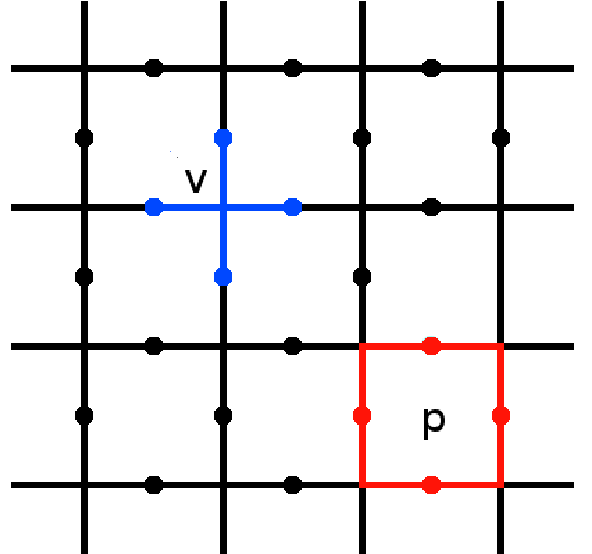
\includegraphics[width=0.5\linewidth]{ToricCodeLattice}
		\caption{Toric Code Lattice}
		\label{fig:toriccodelattice}
	\end{figure}
	
	The solution to this comes from the fact that the V and P operators are mutually commuting. $\sigma_z$ commutes with $\sigma_z$ so the P's commute, and $\sigma_x$ commutes with $\sigma_x$ so the V's commute. If a V and a P are far apart, they will act on different spins, so they will commute or they will share precisely 2 spins. If they share 2 spins a $\sigma_z$ commuting past a $\sigma_x$ will produce a sign, but that happens twice therefore all of these operators commute.
		
The second condition is that the operators only have eigenvalues of $\pm 1 $. This means that since each operator commutes with the Hamiltonian, every ground state must have P=V=1. This does not mean we've pinned
down the ground state yet. Now Euler's characteristic is $\#v-\#e+\#p = 0$ for any graph on a torus, where $\#v$ is the number of verticies, $\#p$ is the number of plaquettes and $\#e$ is the number of edges (links). That means that we have $ 2^{\#e} $ degrees of freedom since there is a spin on each edge but we have $2^(\#v+\#p)$ number of constraints, except that on a torus that overcounts by $2^2$, coming from the fact that $ \prod_v V_v =1 $ and $ \prod_p P_p =1 $ since every spin get's hit twice by a $ sigma_x $,squaring to 1, and twice by a $sigma_z$ term also squaring to 1. This means the total left over degrees of freedom is $ 2^(\#e-\#v-\#p+2) $ which is $2^(2)=4$. This means on a torus, even with those constrains, there is a ground state degeneracy of 4. This ground state degeneracy is a common thing in topological phases. 

The excitations are quiet simple, just have any V or P = -1. Now in order to flip the sign of a P term, we need to flip one of the spins on a vertex, but that spin is also attached to another vertex. This means flipping a spin creates two vertex excitations. If we try to flip another spin to undo one of them, we run into the same problem, we would add a sign to one vertex, and another too a second, which would only move the excitation around. In this sense, excitations can only be created in pairs, and can visualize a string of $\sigma_x$ operators connecting the two excitations. You can close the loop and annihilate the two excitations, leaving the state back in the ground state. Likewise, to flip the sign of the plaquette operator, you just need to apply a $sigma_z$, and the same string argument follows. If you apply a $sigma_y$ operator, you just get a pair of both the vertex and the plaquette excitations. The symbols for these quasiparticles are called e,m and $\psi$